\hypertarget{widgets-2}{%
\section{Widgets (2)}\label{widgets-2}}

\hypertarget{gtktextview-gtktextbuffer-and-gtkscrolledwindow}{%
\subsection{GtkTextView, GtkTextBuffer and
GtkScrolledWindow}\label{gtktextview-gtktextbuffer-and-gtkscrolledwindow}}

\hypertarget{gtktextview-and-gtktextbuffer}{%
\subsubsection{GtkTextView and
GtkTextBuffer}\label{gtktextview-and-gtktextbuffer}}

GtkTextView is a widget for multi-line text editing. GtkTextBuffer is a
text buffer which is connected to GtkTextView. See the sample program
\passthrough{\lstinline!tfv1.c!} below.

\begin{lstlisting}[language=C, numbers=left]
#include <gtk/gtk.h>

static void
app_activate (GApplication *app, gpointer user_data) {
  GtkWidget *win;
  GtkWidget *tv;
  GtkTextBuffer *tb;
  gchar *text;

  text =
      "Once upon a time, there was an old man who was called Taketori-no-Okina. "
      "It is a japanese word that means a man whose work is making bamboo baskets.\n"
      "One day, he went into a mountain and found a shining bamboo. "
      "\"What a mysterious bamboo it is!,\" he said. "
      "He cut it, then there was a small cute baby girl in it. "
      "The girl was shining faintly. "
      "He thought this baby girl is a gift from Heaven and took her home.\n"
      "His wife was surprized at his tale. "
      "They were very happy because they had no children. "
      ;
  win = gtk_application_window_new (GTK_APPLICATION (app));
  gtk_window_set_title (GTK_WINDOW (win), "Taketori");
  gtk_window_set_default_size (GTK_WINDOW (win), 400, 300);

  tv = gtk_text_view_new ();
  tb = gtk_text_view_get_buffer (GTK_TEXT_VIEW (tv));
  gtk_text_buffer_set_text (tb, text, -1);
  gtk_text_view_set_wrap_mode (GTK_TEXT_VIEW (tv), GTK_WRAP_WORD_CHAR);

  gtk_window_set_child (GTK_WINDOW (win), tv);

  gtk_widget_show (win);
}

int
main (int argc, char **argv) {
  GtkApplication *app;
  int stat;

  app = gtk_application_new ("com.github.ToshioCP.tfv1", G_APPLICATION_FLAGS_NONE);
  g_signal_connect (app, "activate", G_CALLBACK (app_activate), NULL);
  stat = g_application_run (G_APPLICATION (app), argc, argv);
  g_object_unref (app);
  return stat;
}
\end{lstlisting}

Look at line 25. A GtkTextView instance is created and its pointer is
assigned to \passthrough{\lstinline!tv!}. When the GtkTextView instance
is created, a GtkTextBuffer instance is also created and connected to
the GtkTextView automatically. ``GtkTextBuffer instance'' will be
referred to simply as ``GtkTextBuffer'' or ``buffer''. In the next line,
the pointer to the buffer is got and assigned to
\passthrough{\lstinline!tb!}. Then, the text from line 10 to 20 is
assigned to the buffer.

GtkTextView has a wrap mode. When it is set to
\passthrough{\lstinline!GTK\_WRAP\_WORD\_CHAR!}, text wraps in between
words, or if that is not enough, also between graphemes.

In line 30, \passthrough{\lstinline!tv!} is added to
\passthrough{\lstinline!win!} as a child.

Now compile and run it.

\begin{figure}
\centering
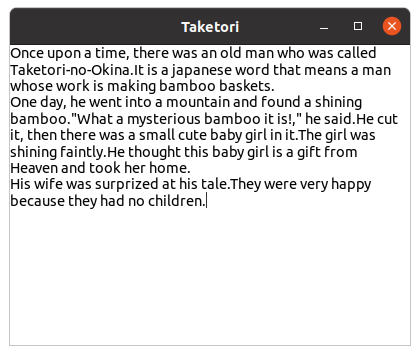
\includegraphics[width=6.3cm,height=5.325cm]{../image/screenshot_tfv1.png}
\caption{GtkTextView}
\end{figure}

There's an I-beam pointer in the window. You can add or delete any
characters on the GtkTextView, and your changes are kept in the
GtkTextBuffer. If you add more characters beyond the limit of the
window, the height increases and the window extends. If the height gets
bigger than the height of the display screen, you won't be able to
control the size of the window, and change it back to the original size.
This is a problem and shows that there is a bug in our program. This can
solve it by adding a GtkScrolledWindow between the GtkApplicationWindow
and GtkTextView.

\hypertarget{gtkscrolledwindow}{%
\subsubsection{GtkScrolledWindow}\label{gtkscrolledwindow}}

What we need to do is:

\begin{itemize}
\tightlist
\item
  Create a GtkScrolledWindow and insert it as a child of the
  GtkApplicationWindow; and
\item
  Insert the GtkTextView widget to the GtkScrolledWindow as a child.
\end{itemize}

Modify \passthrough{\lstinline!tfv1.c!} and save it as
\passthrough{\lstinline!tfv2.c!}. The difference between these two files
is small.

\begin{lstlisting}
$ cd tfv; diff tfv1.c tfv2.c
5a6
>   GtkWidget *scr;
24a26,28
>   scr = gtk_scrolled_window_new ();
>   gtk_window_set_child (GTK_WINDOW (win), scr);
> 
30c34
<   gtk_window_set_child (GTK_WINDOW (win), tv);
---
>   gtk_scrolled_window_set_child (GTK_SCROLLED_WINDOW (scr), tv);
40c44
<   app = gtk_application_new ("com.github.ToshioCP.tfv1", G_APPLICATION_FLAGS_NONE);
---
>   app = gtk_application_new ("com.github.ToshioCP.tfv2", G_APPLICATION_FLAGS_NONE);
\end{lstlisting}

Here is the complete code of \passthrough{\lstinline!tfv2.c!}.

\begin{lstlisting}[language=C, numbers=left]
#include <gtk/gtk.h>

static void
app_activate (GApplication *app, gpointer user_data) {
  GtkWidget *win;
  GtkWidget *scr;
  GtkWidget *tv;
  GtkTextBuffer *tb;
  gchar *text;

  text =
      "Once upon a time, there was an old man who was called Taketori-no-Okina. "
      "It is a japanese word that means a man whose work is making bamboo baskets.\n"
      "One day, he went into a mountain and found a shining bamboo. "
      "\"What a mysterious bamboo it is!,\" he said. "
      "He cut it, then there was a small cute baby girl in it. "
      "The girl was shining faintly. "
      "He thought this baby girl is a gift from Heaven and took her home.\n"
      "His wife was surprized at his tale. "
      "They were very happy because they had no children. "
      ;
  win = gtk_application_window_new (GTK_APPLICATION (app));
  gtk_window_set_title (GTK_WINDOW (win), "Taketori");
  gtk_window_set_default_size (GTK_WINDOW (win), 400, 300);

  scr = gtk_scrolled_window_new ();
  gtk_window_set_child (GTK_WINDOW (win), scr);

  tv = gtk_text_view_new ();
  tb = gtk_text_view_get_buffer (GTK_TEXT_VIEW (tv));
  gtk_text_buffer_set_text (tb, text, -1);
  gtk_text_view_set_wrap_mode (GTK_TEXT_VIEW (tv), GTK_WRAP_WORD_CHAR);

  gtk_scrolled_window_set_child (GTK_SCROLLED_WINDOW (scr), tv);

  gtk_widget_show (win);
}

int
main (int argc, char **argv) {
  GtkApplication *app;
  int stat;

  app = gtk_application_new ("com.github.ToshioCP.tfv2", G_APPLICATION_FLAGS_NONE);
  g_signal_connect (app, "activate", G_CALLBACK (app_activate), NULL);
  stat = g_application_run (G_APPLICATION (app), argc, argv);
  g_object_unref (app);
  return stat;
}
\end{lstlisting}

Compile and run it. Notice how this time the window doesn't extend when
you type a lot of characters, it just scrolls and displays a slider.
